% Options for packages loaded elsewhere
\PassOptionsToPackage{unicode}{hyperref}
\PassOptionsToPackage{hyphens}{url}
%
\documentclass[
]{book}
\usepackage{amsmath,amssymb}
\usepackage{iftex}
\ifPDFTeX
  \usepackage[T1]{fontenc}
  \usepackage[utf8]{inputenc}
  \usepackage{textcomp} % provide euro and other symbols
\else % if luatex or xetex
  \usepackage{unicode-math} % this also loads fontspec
  \defaultfontfeatures{Scale=MatchLowercase}
  \defaultfontfeatures[\rmfamily]{Ligatures=TeX,Scale=1}
\fi
\usepackage{lmodern}
\ifPDFTeX\else
  % xetex/luatex font selection
\fi
% Use upquote if available, for straight quotes in verbatim environments
\IfFileExists{upquote.sty}{\usepackage{upquote}}{}
\IfFileExists{microtype.sty}{% use microtype if available
  \usepackage[]{microtype}
  \UseMicrotypeSet[protrusion]{basicmath} % disable protrusion for tt fonts
}{}
\makeatletter
\@ifundefined{KOMAClassName}{% if non-KOMA class
  \IfFileExists{parskip.sty}{%
    \usepackage{parskip}
  }{% else
    \setlength{\parindent}{0pt}
    \setlength{\parskip}{6pt plus 2pt minus 1pt}}
}{% if KOMA class
  \KOMAoptions{parskip=half}}
\makeatother
\usepackage{xcolor}
\usepackage{longtable,booktabs,array}
\usepackage{calc} % for calculating minipage widths
% Correct order of tables after \paragraph or \subparagraph
\usepackage{etoolbox}
\makeatletter
\patchcmd\longtable{\par}{\if@noskipsec\mbox{}\fi\par}{}{}
\makeatother
% Allow footnotes in longtable head/foot
\IfFileExists{footnotehyper.sty}{\usepackage{footnotehyper}}{\usepackage{footnote}}
\makesavenoteenv{longtable}
\usepackage{graphicx}
\makeatletter
\def\maxwidth{\ifdim\Gin@nat@width>\linewidth\linewidth\else\Gin@nat@width\fi}
\def\maxheight{\ifdim\Gin@nat@height>\textheight\textheight\else\Gin@nat@height\fi}
\makeatother
% Scale images if necessary, so that they will not overflow the page
% margins by default, and it is still possible to overwrite the defaults
% using explicit options in \includegraphics[width, height, ...]{}
\setkeys{Gin}{width=\maxwidth,height=\maxheight,keepaspectratio}
% Set default figure placement to htbp
\makeatletter
\def\fps@figure{htbp}
\makeatother
\setlength{\emergencystretch}{3em} % prevent overfull lines
\providecommand{\tightlist}{%
  \setlength{\itemsep}{0pt}\setlength{\parskip}{0pt}}
\setcounter{secnumdepth}{5}
\usepackage{booktabs}
\usepackage{amsthm}
\makeatletter
\def\thm@space@setup{%
  \thm@preskip=8pt plus 2pt minus 4pt
  \thm@postskip=\thm@preskip
}
\makeatother
\ifLuaTeX
  \usepackage{selnolig}  % disable illegal ligatures
\fi
\usepackage[]{natbib}
\bibliographystyle{apalike}
\IfFileExists{bookmark.sty}{\usepackage{bookmark}}{\usepackage{hyperref}}
\IfFileExists{xurl.sty}{\usepackage{xurl}}{} % add URL line breaks if available
\urlstyle{same}
\hypersetup{
  pdftitle={Competition and Regulation in the AI Era},
  pdfauthor={Manav Adwani, Sohil Apte, Lauren Brown, Anson Lee, Xuexin Li},
  hidelinks,
  pdfcreator={LaTeX via pandoc}}

\title{Competition and Regulation in the AI Era}
\author{Manav Adwani, Sohil Apte, Lauren Brown, Anson Lee, Xuexin Li}
\date{2023-08-20}

\begin{document}
\maketitle

{
\setcounter{tocdepth}{1}
\tableofcontents
}
\hypertarget{introduction}{%
\chapter{Introduction}\label{introduction}}

From assisting with strategy to generating content, artificial intelligence (AI) is already influencing how businesses operate. The consulting firm Accenture projects an average profitability boost of 38\% by 2035 across sixteen major industries. Additionally, AI has led to increased productivity and reduced costs, particularly in analytics, product development, and customer service. This has led many businesses to adopt AI with large firms like Google and Microsoft potentially investing billions in the technology. It is apparent that AI will provide a new arena for businesses to compete in.

Yet, the excitement over the benefits of AI has yielded challenges for businesses and regulators. For businesses, there are questions on what duties to assign AI. One of the causes of the ongoing actor and writer strikes is concerns over AI replacing human workers. Technology contractors in the Republic of Kenya are suing Meta for being exposed to psychologically damaging content while moderating its generative AI systems. Additionally, the exact information necessary for AI to arrive at optimal solutions is not known. Recent studies have shown there are limits to the effectiveness of pricing algorithms and that data reaches a point of diminishing returns. AI has also proven to be difficult to regulate; governments and institutions face the challenge of controlling something without knowing its full potential. The laws they establish will inevitably provide another dimension to business competition.

As businesses adopt AI, it is crucial to consider both the benefits and challenges to best predict its impact on the competitive landscape. To what degree will businesses rely on these systems and how will their competitors respond? What industries are likely to see the most meaningful change in operations? And what does this mean for the workers within those industries? Acknowledging these questions is the key to developing a business environment that utilizes AI in an efficient, fair, and ethical manner.

\hypertarget{about-us}{%
\chapter{About Us}\label{about-us}}


\includegraphics{images/MBAngels.jpg}

\hypertarget{mbangels}{%
\section{MBAngels}\label{mbangels}}

We are a team of Master of Business Analytics (MBAn) students with the goal of understanding how the new age of generative artificial intelligence (AI) will impact the world, and specifcally, impact our cohort as analytics students. By combining our wide array of backrounds, diverse skillsets, and range of persepctives, we hope to compile a robust report that captures the impact AI will have on all levels of industry.

\hypertarget{manav-adwani}{%
\section{Manav Adwani}\label{manav-adwani}}

\textbf{Background:}
Manav studied commerce in his undergrad and comes from a family business background. After completing a relatively generic degree for his undergrad, he now wants to explore the true power of business when data analytics is applied to it. This would include learning more about the strategy side of analytics.

\textbf{Experience:}
While he is enthusiastic about learning the technical aspect, he hopes to provide an in depth business perspective to the team. The team can benefit from his experience in EY and his knowledge about setting up and running a successful international business as an entrepreneur.

\hypertarget{sohil-apte}{%
\section{Sohil Apte}\label{sohil-apte}}

\textbf{Background:}
Sohil is originally from Canton Ma, and graduated from the University of Michigan in 2023. With a BS in Computer Science and a concentration on artificial intelligence and machine learning, Sohil has a robust theoretical perspective of AI, and an understanding of the intricacies of machine learning applications.

\textbf{Experience:}
As a former Computer Science student with practical experience as a Software/Machine Learning Engineer at a startup, his knowledge of machine learning model development and deployment, along with its business implications, offers insights into the real-world competitive impact of AI technologies.

\hypertarget{lauren-brown}{%
\section{Lauren Brown}\label{lauren-brown}}

\textbf{Background:}
Lauren is from Brighton, Michigan and graduated from the school of LSA at the University of Michigan in 2023. Being a Psychology major, Lauren is interested in society's reaction to AI and its outcomes.

\textbf{Experience:}
Lauren has experience in marketing, and has developed a passion for AI regulation as she recognized the potential for AI's powerful impact on the industry alongside the need for ethical guidelines to protect consumers and ensure fair practices.

\hypertarget{anson-lee}{%
\section{Anson Lee}\label{anson-lee}}

\textbf{Background:}
Anson Lee is originally from Poughkeepsie, New York. He graduated with a BBA from the Ross School of Business in 2023.

\textbf{Experience:}
His experience includes working in the operations departments of Goldman Sachs and Toyoda Gosei North America. He is also an avid cinephile and skier. Anson Lee is primarily concerned with how AI will be regulated to protect workers and industries.

\hypertarget{xuexin-li}{%
\section{Xuexin Li}\label{xuexin-li}}

\textbf{Background:}
Xuexin is originally from Beijing, China. Xuexin studied in Business Management and Economics at UC Santa Cruz during her undergraduate years.

\textbf{Experience:} Xuexin has immersed herself in the Digital Marketing industry in China after graduation. Her experience has sparked a deep interest in exploring AI's transformative potential in reshaping marketing strategies and consumer behavior.

Our combined skills and shared passion for the topic make us uniquely equipped to tackle the questions surrounding AI and the impacts it will have on comeptition and strategy. We are excited to share our research and insights in this paper.

\hypertarget{impact-of-ai-on-the-competitive-landscape}{%
\chapter{Impact of AI on the Competitive Landscape}\label{impact-of-ai-on-the-competitive-landscape}}

\hypertarget{feedback-loop}{%
\section{``Feedback Loop''}\label{feedback-loop}}

From customer-targeted advertisements to automated chatbots, AI has found its place in every industry. The excellence of a modern business is often synonymous with the use of AI and related systems in its day-to-day operations. While AI is used in the back end and the front end, it is the customer-centric application of AI that helps businesses to gain a competitive advantage in any industry.

A common misconception is that accessibility to data drives competitive advantages for businesses. Even regulators share the perspective that companies amassing large amounts of data can pose barriers for new entrants (Iansiti, 2021). The main concern is that the availability of excess data can result in a ``feedback loop''.

A feedback loop is formed when the companies with the most data use it to reinforce their decisions and deliver heightened value to their customers. As they grow their customer share, these companies inherit access to even more data, which can be used to make additional derivations. This is particularly true for younger companies, as acquiring data is a useful tool for building the user base necessary to take advantage of network effects. However, deeper research shows that this might not be the case for more mature firms, because the accumulation of data eventually yields diminishing returns. This is especially true when data lacks quality, scalability, or cannot be combined with complementary data. Also important is the degree to which data is exclusive and inimitable. This prevents rival firms from nullifying a data advantage through their own usage. For example, streaming services have been able to use similar data to Netflix to reduce its competitive data advantage. Clearly, the positive feedback loop is not infinite, and the usefulness of data has an implicit ceiling, making it a nuanced issue for regulators to tackle.

\hypertarget{competitive-ai-across-industries}{%
\section{Competitive AI Across Industries:}\label{competitive-ai-across-industries}}

With the mass adoption of AI by businesses, it was inevitable firms would attempt to achieve a competitive advantage via this technology. Applications for reducing cost and maximizing value have manifested across a diverse set of industries. However, the wide range of use cases makes it difficult to understand the complete effect of AI on the competitive relationship between businesses. Already, businesses use AI in a plethora of frontstage functions that are relevant for the consumers interacting with them and the workers that design them. Below are examples of some of the most significant users of AI technology:

\hypertarget{media}{%
\section{Media}\label{media}}

Perhaps no industry is more concerned with its front-stage activities than the media industry. With the success of their products and services depending mainly on consumer perceptions, it makes sense for firms within the industry to utilize new technology to help ensure success. Even in its current state, AI is capable of generating content for media firms (Global Artificial Intelligence, 2019). It could also be used to modify existing content, through methods such as mimicking actor's performances in a foreign language (Toonkel, Sharma, 2023).

AI could also be implemented in other front-stage functions. HBO has held discussions with OpenAI about the potential for using AI-generated descriptions of shows to display online (Toonkel, Sharma, 2023). Within streaming sites, the technology also has the ability to curate the user experience through recommendation algorithms. This has the benefit of creating individual user profiles that can be used as the basis for delivering the necessary content to attract and retain users.

However, the potential usage of AI has garnered massive backlash within the media industry. The ongoing writers' and actors' strikes were in part caused by the fear that the technology would claim jobs and justify worsened working conditions. The challenge for leaders and workers within the media industry for the foreseeable future will be to settle on agreements regulating artificial intelligence usage. This will be key in leveraging the benefits of the technology while ensuring the industry can maintain relationships with its partners.

\hypertarget{tech}{%
\section{Tech}\label{tech}}

The technology industry has been leveraging advancements in AI to assist in the innovative process. Firms are using this technology to create customer personas and create front stage systems, such as user interfaces, optimized through AI. The collection of data also helps technology firms design products better suited to customer demands, which has the potential to drive significant sales (Global Artificial Intelligence, 2019). The success of these data-driven initiatives has led firms to attempt to collect as much data as possible, but some studies have suggested that this activity eventually leads to diminishing returns.

Strategy in tech must be based on the quality and relativity of the data rather than just on the volume of data. In the tech industry, research has shown that the use of deep learning is much more accurate where the data sets are massive. However, research shows that this might not always be true. Herein, the systems developed to articulate data find it difficult to make any sense of ``start data''. This data is often referred to as cold data which is too small to derive any meaningful explanation. However, as more data comes in, generally referred to as the ``power-law'' data, each additional data point helps to improve the performance of the algorithm. After a point, any additional data will not be of significant help to the algorithm (Iansiti, 2021).

\hypertarget{retail}{%
\section{Retail}\label{retail}}

In the retail industry, artificial intelligence is being utilized for customer-centered strategy. This would mean the use of various front-end targeting mechanisms such as the dynamic pricing mechanism, customer centric assortment optimization, and demand forecasting and planning. Dynamic pricing also works in tandem with the promotion optimization algorithm which helps determine what promotions should reach which customers (Hetu, 2022). AI is also increasingly leveraged in the Best-Fit Apparel algorithm which facilitates the customer in buying according to their style. It is evident that in order to stay competitive in the retail industry, companies must facilitate their operations through AI.

This system is especially important in e-commerce due to the previously mentioned feedback loop. To attract enough users to sustain the business, firms like Amazon and Alibaba invest in them to attract users. As more buyers and sellers utilize their platforms, the feedback loop begins as new sources of data are now available. This is in part what makes e-commerce firms successful. Having consumer data they can analyze with AI and market accordingly.

One of the most effective ways retail businesses deploy AI is by upselling and cross-selling. These AI systems also have the benefit of being relatively easy to implement. In e-commerce, algorithms can be used to detect a competitor's price and adjust one's own accordingly (Hamer, Elliot, Hare, 2023). AI pricing is not limited only to online retailers though. Walmart has been testing robots that scan shelves to calculate stock and determine prices accordingly. In addition to serving as an example of price management, this system also shows how AI can limit the burden of work on employees who are now free to focus more on curating the in-store customer experience (Global Artificial Intelligence, 2019).

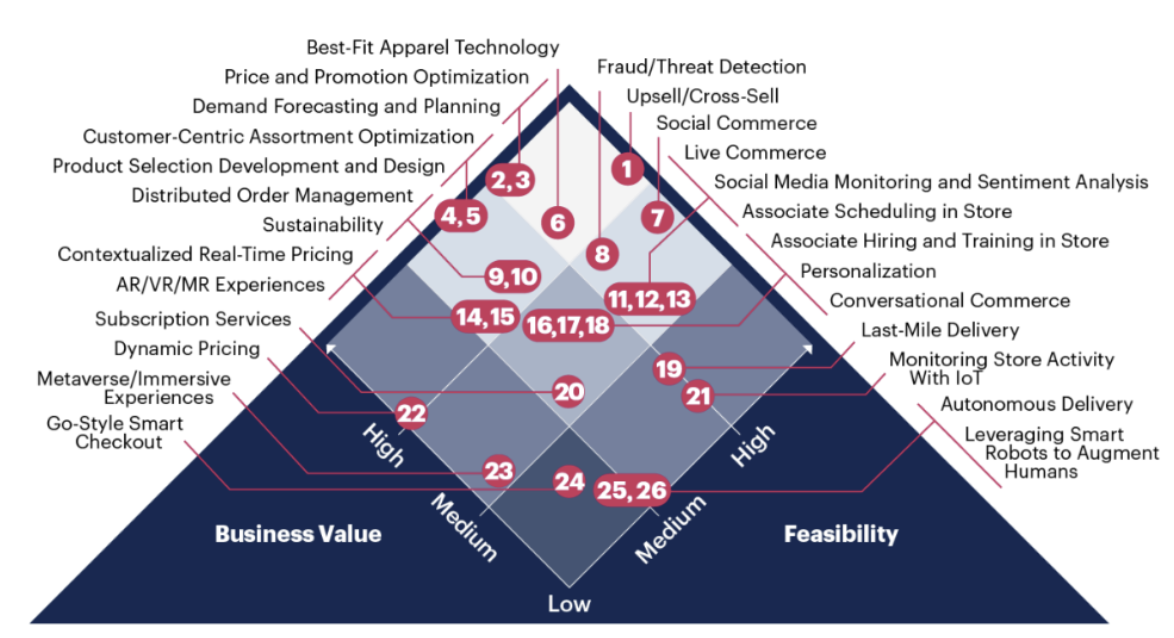
\includegraphics{images/retailimage.png}
\#\# Applications of AI

\hypertarget{customer-service}{%
\section{Customer Service}\label{customer-service}}

``AI can help to improve customer service by automating routine tasks and providing personalized recommendations.''
Satya Nadella, CEO of Microsoft

AI has already made significant inroads into customer service, with tools like chatbots and virtual assistants taking on a variety of customer-related tasks. Industry experts are predicting a number of trends in this area. The adoption of AI-powered chatbots is set to rise, with the global chatbot market projected to reach a substantial USD 27,297.2 million by 2030. This growth is expected to occur at a compound annual rate of 23.3\% from 2023 to 2030. (Taylor, 2023) The advantages of chatbots are 24/7 availability and efficient handling of inquiries compared to human representatives. As chatbots continue to evolve, they are becoming increasingly sophisticated, capable of addressing both straightforward queries and complex issues. This advancement is proving to be important for customer service teams seeking streamlined interactions.

The progression of AI is also leading to a shift towards more personalized customer experiences. Insights from the State of AI report underscore that people are growing more comfortable with AI's ability to offer personalized messages (50\%) and tailored experiences (46\%) (Taylor, 2023). Leveraging customer data, AI is now capable of providing customized product recommendations and interactions that enrich the overall customer journey.

Furthermore, AI's predictive capabilities are expected to become more advanced. With enhanced accuracy, AI will be able to predict customer behaviors with precision, resulting in improved customer experiences and heightened satisfaction levels. For instance, AI systems can anticipate when a customer is likely to make a purchase based on their historical behavior and interactions. This predictive ability opens the door for timely actions, such as delivering personalized offers at opportune moments.

Debates about AI's role in customer service will continue. While some analysts envision AI completely replacing human representatives, others anticipate a collaborative relationship between AI and human agents. Research data indicates that by 2024, approximately 61\% of customer service professionals will rely on AI or other automated processes. (Taylor, 2023) Although AI excels at handling a diverse range of queries, situations demanding human empathy and understanding are expected to persist. These ongoing discussions reflect the evolving landscape of customer service and the dynamic interplay between technology and human expertise.

\hypertarget{marketing}{%
\section{Marketing}\label{marketing}}

``As AI continues to evolve, we can expect to see more intelligent automation in marketing, making it easier and faster to reach our audience. The possibilities are endless, and the future of marketing looks very exciting.''
Neil Patel, Co-founder of NP Digital

The future of AI in marketing holds transformative potential across a range of aspects, extending from enhancing customer engagement to refining content creation strategies. Marketers are actively exploring innovative methods to interact with consumers and leverage the capabilities of AI to their advantage. However, there are disparities in the advancement of this industry, with larger corporations leading AI integration due to their substantial resources and expertise.

Moving into the next decade, substantial advancements and challenges are anticipated in the realm of AI marketing. Firstly, the analysis of consumer behavior through AI-driven methods presents a valuable opportunity for gaining accurate insights into data. This allows marketers to identify trends, optimize their campaigns, and track the return on investment based on a more personalized comprehension of their customers. The potential for real-time inferencing support through AI-powered analytic tools further enhances the effective utilization of consumer data (Wolinsky, 2023).

Moreover, advanced AI systems are positioned to process vast quantities of customer data, interpreting emerging patterns and predicting their evolution in real time (Wolinsky, 2023). This predictive analysis will significantly refine marketing campaigns, granting marketers a higher level of precision when evaluating the effectiveness of their efforts.

Addressing the growing demand for personalized content curation, AI-powered tools are on the rise. These tools can efficiently curate content tailored to specific platforms and products, resulting in reduced lead times and heightened execution accuracy (Wolinsky, 2023). This shift empowers marketers to attain more measurable outcomes, make strategic adjustments, and effectively engage their target audiences.

With the ongoing digital transformation, the need for dependable on-demand customer service has experienced a sharp and significant increase. While automated solutions like chatbots have improved response times, challenges persist in effectively resolving customer concerns. Ongoing development in natural language processing (NLP) models is set to bridge this gap, enhancing the capacity of automated systems to understand and address complex customer queries (Wolinsky, 2023).

Voice recognition technology, in conjunction with AI applications such as Alexa and Siri, is expected to elevate the role of language in marketing. Real-time applications of these technologies can optimize voice searches and enhance the comprehension of natural language, thereby fostering improved communication and engagement with consumers (Wolinsky, 2023). AI-driven automation is set to revolutionize digital marketing workflows. It can improve productivity, manage project deliveries, enhance market insights, and generate more personalized messaging. However, AI does not replace human creativity, which is still essential for the successful execution of these strategies.

\hypertarget{talent-management}{%
\section{Talent Management}\label{talent-management}}

``Cognitive computing is going to be the next big thing in human resource management. It is going to transform how we hire, train, and retain employees.''
- Ginni Rometty, Former CEO of IBM

Generative AI has the potential to transform recruiting by assisting managers in creating better job requirements and personalizing outreach to candidates. It can identify the skills needed for success in a job, which improves both the speed and quality of the process. Organizations currently struggle to personalize outreach to a large number of applicants. AI can also enhance candidate outreach and communication, making it easier to provide important information to applicants in a more personalized manner (Hancock, 2023).

``With generative AI, you can include much more personalization about the candidate, the job, and what other jobs may be available if there's a reason the applicant isn't a fit. All those things are made immensely easier and faster through generative AI.''
- Bryan Hancock

AI's role in talent evaluation is equally significant, as it can accelerate the shift from credentials to skills-based assessment (Hancock, 2023). The technology's ability to tag unstructured data for keywords can help identify relevant capabilities and skills, enabling a more inclusive and skills-based approach to candidate evaluation, enriching the pool of potential candidates and promoting a more comprehensive view of skills.

Beyond the initial recruitment phase, AI-driven career development assistance emerges as a valuable resource for employees seeking to navigate their professional paths (Hancock, 2023). AI-powered assistants can guide individuals by offering insights into potential career opportunities, identifying role models, and highlighting necessary skills for advancement. This dynamic interaction facilitates informed decision-making and strategic planning for career growth.

While AI's potential is considerable, its role in performance review processes is complex. Although AI could play a role in drafting initial performance reviews based on aggregated feedback, the importance of human judgment and empathy in finalizing these reviews remains undeniable (Schaninger, 2023). This emphasizes the interplay between technological support and the inherently human elements of feedback and assessment.

As organizations adopt generative AI tools, leaders need to consider the impact on workflows, collaboration models, and job roles. Proper change management strategies should be employed to maximize the benefits of the technology without disrupting the work ecosystem (Yee, 2023).

``The other thing is there's a real opportunity for what we typically call `change
management.' If you don't think through how the technology changes the job, workflow,
or collaboration model, then you're not necessarily directing that additional time toward
something that's more value added.''
- Lareina Yee

\hypertarget{major-players-use-of-ai}{%
\section{Major Players' Use of AI:}\label{major-players-use-of-ai}}

\hypertarget{alibaba}{%
\subsection{Alibaba:}\label{alibaba}}

\hypertarget{amazon}{%
\subsection{Amazon:}\label{amazon}}

\hypertarget{starbucks}{%
\subsection{Starbucks:}\label{starbucks}}

\hypertarget{regulation-of-ai}{%
\chapter{Regulation of AI}\label{regulation-of-ai}}

AI technology has been making major advances with AI systems, such as ChatGPT, being used by over 40\% of college students in the United States (Balderson, 2023). Companies and organizations all around the world are increasing their use of AI to gain a competitive advantage in their respective industries. This race of AI technology is putting focus on what regulation needs to be developed to control these advances. AI is becoming a core part of political discourse, and big names in the tech industry such as Steve Wozniak, Elon Musk, and politicians such as Andrew Yang, have signed an open letter asking for a moratorium on AI experimentation for regulation development (Pause Giant AI experiments: An open letter, 2023). While this open letter has not led to any action, it does bring attention to the fact that governments will have to focus a large part of their future legislation on regulation. AI systems and regulations are global and inter-industry issues. There are so many different pieces, in different industries, and they're all moving at different paces, which makes it difficult to legislate.

\hypertarget{current-regulation}{%
\section{Current regulation}\label{current-regulation}}

Governments around the world have only scratched the surface on legislating AI regulation. Most countries, like the United States, are still debating what parts of AI should be regulated, and how much regulation is appropriate. There are a few exceptions to this trend. The European Parliament has recently taken its first step to legal regulation by passing a draft law named the AI Act. This act will focus on limiting the most high-risk parts of AI technology, such as facial recognition. It will also force upcoming AI systems to be more open about the data they are using. While this is only a draft law, the final version of this law is expected to be passed by the end of 2023, making it one of the first large steps toward government-enforced AI regulation (Satariano, 2023).

\hypertarget{proposed-regulation}{%
\section{Proposed regulation}\label{proposed-regulation}}

AI regulations are slowly starting to be put into effect, but there are still so many questions on how it will work. The CEO of OpenAI, Sam Altman, wrote a testimony to the Senate this May asking that they start strongly considering regulating artificial intelligence (Hendrix, 2023). He proposed solutions such as licensing companies to use AI, or creating a government agency strictly responsible for AI regulation. Altman's solutions were questioned by some, though, as there are still many disagreements about what the best way to legislate AI should be. While these solutions seem good on paper, the answer to how to regulate AI is not that simple. Officials are predicting that AI regulation agencies have the potential of being compromised. Having only one small sector of government responsible for such a broad and important issue could lead to bias. Experts have recommended that AI needs to be diversely regulated by a combination of different agencies and organizations. They have said that regulation should be created by a collaboration from academia, policy experts, industry experts, and even international agencies (Susarla, 2023).

New strategies for AI regulation are being proposed regularly by CEOs and other big names in the tech field. AI technology is progressing rapidly and there is an understanding of the need to regulate it before it gets bigger, faster, and stronger. While most tech officials are in agreement about the importance of regulation, government officials can often be harder to come by. The median age of the U.S. The House of Representatives is 58 years old, and the median age is 65 years old in the Senate. The United States lawmaker demographic is much older than the mean age in America (38 years old) (Blazina and DeSilver, 2023). Their age could mean they have lesser knowledge or insight into these new technological advancements than young, up-and-coming workers in the tech industry do. The lawmakers' lack of understanding of artificial intelligence applications can lead to more debate than needed on what type of regulation should be established.

These are prime years to establish effective regulations on artificial intelligence and how it is used. Setting regulations now, when AI is not overwhelmingly powerful, could be key to getting a grasp on this technology and its future that we cannot predict. Some places, like the European Union, are taking their first steps toward government action, but others, like the United States, have barely scratched the surface. While companies are already beginning to integrate AI regulation into their business, not every organization will follow suit without government intervention. AI Regulation should be expected to be a hot topic in government and politics in the near future since AI will continue to progress and the demand for regulation will increase with it.

\hypertarget{regulation-as-a-competitive-advantage}{%
\section{Regulation as a competitive advantage}\label{regulation-as-a-competitive-advantage}}

AI use within companies is becoming increasingly normalized in numerous industries - leading to a higher mistrust in AI and AI regulation among customers and employees of these companies. So much of what artificial intelligence is can be difficult for the average individual to grasp. For some people, the first thing they think of when they hear ``AI'' is horror stories of technology taking over the world. Acknowledging these individuals and understanding their views is a step that some companies have already started to take.

\hypertarget{pros}{%
\subsection{Pros}\label{pros}}

Responsible AI is a process that certain companies have acquired to regulate their own use of AI. It is the process of developing AI systems that minimizes biases, enforces data security, ensures transparency within companies, and creates opportunities for employees to speak out on their concerns on AI use. Companies using this form of AI regulation have actually found that it can be used as a competitive advantage. Currently, 36\% of organizations have said they believe it will create opportunities for competitive differentiation (Eitel-Porter, 2023). The ability to deliver trustworthy AI systems that are regulation-ready can help a company attract new customers because they are using AI safely and are being transparent about its use. While this is a step in the right direction, AI regulation needs to be supported by governments to truly make a difference.

\hypertarget{cons}{%
\subsection{Cons}\label{cons}}

While there are obvious benefits to regulating the use of AI, there are also a number of setbacks that could have a negative effect. Limiting its capabilities or room for growth could lead to artificial intelligence not having the ability or flexibility to adapt or learn in positive ways. Strict regulations could restrain creativity and innovation, and lessen the amount of risks taken by companies. This also could become a problem in relation to international affairs. Companies within countries that set stricter regulations will suffer in comparison to companies rooted in countries that have more flexible AI control (Balderson, 2023).

\hypertarget{the-value-of-a-ross-mban}{%
\chapter{The Value of a Ross MBAn}\label{the-value-of-a-ross-mban}}


\includegraphics{images/RossStudentsPhoto.jpg}

\hypertarget{blending-technical-skills-with-business-skills}{%
\section{Blending technical skills with business skills}\label{blending-technical-skills-with-business-skills}}

As AI changes the business landscape, Master of Business Analytics (MBAn) students, from renowned institutions like the Ross School of Business, will emerge as key players. The MBAn curriculum prepares students with both the technical skills and business acumen to lead in AI-driven business domains. Executives are finding themselves facing a set of realities including untapped opportunity and existential risks (Ransbotham, 2019). As businesses invest in AI-driven operations, students with a strong understanding of technology, strategy, and leadership will be in high demand for executive roles with AI decision making.

\hypertarget{meeting-the-demand-for-ai-proficient-leaders-and-strategists}{%
\section{Meeting the demand for AI-proficient leaders and strategists}\label{meeting-the-demand-for-ai-proficient-leaders-and-strategists}}

The market is craving strong decision-makers with knowledge bases in AI. Although there is a current surplus of technical leaders like software engineers and data scientists, the biggest challenge is finding people with business expertise to contribute to AI strategy. After all, companies cannot solve strategy problems with AI without people who truly understand the underlying business goals at hand. (Yuval, 2023)

\hypertarget{the-ai-landscape-in-corporate-strategy}{%
\section{The AI Landscape in Corporate Strategy}\label{the-ai-landscape-in-corporate-strategy}}

In the current AI landscape, success is derived from harnessing its vast potential to enhance efficiency, foster innovation, and secure a competitive advantage. These advantages can only be realized if executives adopt and scale AI practices in their company in an effective manner.

\hypertarget{cultural-and-structural-obstacles-to-ai-integration}{%
\section{Cultural and Structural Obstacles to AI Integration}\label{cultural-and-structural-obstacles-to-ai-integration}}

The integration of artificial intelligence into the corporate ecosystem is a compelling value proposition for any company. However, only ``8\% of firms engage in core practices that support widespread adoption of AI and advanced analytics (Harvard Business Review, 2020)''. Just ``12\% of the executives and senior executives have included AI initiatives in their corporate strategies.'' (Mostafa, 2023) Even with so much to gain from the integration of AI, many organizations find themselves faced with cultural and structural barriers.

\hypertarget{misperceptions}{%
\subsection{Misperceptions}\label{misperceptions}}

The polarizing nature of the discourse surrounding AI has led to hesitancy in its implementation and adoption. When executives think about automating strategy, many are looking too far ahead, focusing on how AI would completely replace business leaders and their decision-making. Shifting their focus to the use of AI as ``building blocks'' of their corporate strategy could significantly improve their business outcomes (Yuval, 2023). Another misconception is the expectation of instant rewards from AI as simply a plug-and-play solution. Even when AI is adopted as a business strategy, it has a constrained use case, which limits its versatility and curtails its ultimate potential (Harvard Business Review, 2020).

\hypertarget{cultural-reluctance}{%
\subsection{Cultural Reluctance}\label{cultural-reluctance}}

The nuances of human behavior play critical roles in AI's corporate integration. Humans are resistant to change by nature, especially when it disrupts long-established tried and true norms. Changes in a business setting are no exception. Many established organizations operate on top-down decision-making. Transitioning to a model where decisions are reinforced by AI represents an upending structural and cultural shift from intuition-based CEO decision-making to a flattened organizational structure backed by data-reinforced conclusions. (Mostafa, 2023).

Overlaying these challenges is the undercurrent of the fear of the unknown. There is anxiety over job losses and reduced human significance. McKinsey highlights the issue directly: ``The big challenge is finding strategists to contribute to the AI effort. You are asking people to get involved in an initiative that may make their jobs less important (Yuval, 2023).''

\hypertarget{overcoming-barriers-to-entry}{%
\section{Overcoming Barriers to Entry}\label{overcoming-barriers-to-entry}}

Incorporating artificial intelligence into corporate strategy requires a holistic approach. There are key considerations necessary to ensure a smooth transition into an AI-integrated business.

\hypertarget{enhanced-human-ai-interactions}{%
\subsection{Enhanced Human-AI Interactions}\label{enhanced-human-ai-interactions}}

The incorporation of AI into the business world is a symbiotic relationship that demands continual human feedback for improvement (Degnan, 2023). Companies must also embrace diverse teams with varying skills and perspectives to ensure that AI solutions cater to a wide span of organizational needs. After all, the only way to maximize the potential of a data-driven technology like AI is to accommodate it with many diverse inputs (Harvard Business Review, 2020).

\hypertarget{culture-evolution}{%
\subsection{Culture Evolution}\label{culture-evolution}}

Effective implementation of AI in businesses means transitioning the corporate culture to embrace AI rather than just accepting it (Degnan, 2023). In addition to a deliberate reception of AI, an organization's attitude towards its deployment should be dynamic and iterative. By valuing continuous feedback and experimentation, organizations can develop robust AI solutions that can operate at scale. Notably, almost 90\% of companies successful in scaling AI practices allocated more than half of their analytics budgets to adoption-centric activities - emphasizing the importance of company-wide cultural shifts (Harvard Business Review, 2020).

\hypertarget{alignment-with-core-objectives}{%
\subsection{Alignment with Core Objectives}\label{alignment-with-core-objectives}}

AI should resonate with a company's mission and objectives. For example, Southwest Airlines emphasizes low-cost airfare. Their AI strategies amplify those core beliefs and provide customer value consistent with the company's values (Degnan, 2023).

\hypertarget{consistent-evaluation}{%
\subsection{Consistent Evaluation}\label{consistent-evaluation}}

Successful AI integration requires consistent performance monitoring. Companies should develop a robust set of Key Performance Indicators (KPIs) to measure how closely the AIs contributions continue to align with core objectives and provide tangible value (Degnan, 2023).

By addressing these tenets of AI strategy, organizations can pave the way to seamless integration and success - with MBAn students leading the way.

\hypertarget{conclusion}{%
\chapter{Conclusion}\label{conclusion}}

The MBAn student body and the business community as a whole stand on the precipice of a new age of commerce. The benefits provided by AI have allowed firms across numerous industries to improve on their processes both internal and external. According to a global survey by McKinsey, a significant portion of executives from companies that have adopted AI report an increase in revenue in the business areas it influenced. Specifically, 63\% of respondents claimed a revenue boost from AI integration. AI's potential to optimize company-wide operations also translates into significant cost savings. McKinsey's report highlights that 44\% of the executives observed a reduction in costs due to the adoption of AI in their business operations (McKinsey Company, 2019). Business students should consider AI's current impact and its future so they may thrive as tomorrow's leaders. Yet, this is a task easier said than done; with so many industries applying AI in so many ways, it is difficult to understand such a revolutionary technology via a holistic analysis. This report has mainly focused on front-stage elements in a few key industries that individuals are likely to interact with as workers and consumers. It is also important to acknowledge that students are not the only ones struggling to understand the impact of AI. There is an immense need for regulation, and it falls on business leaders informed on the issue to guide governments toward effective policies. This is especially important considering the conflict between managers, workers, and technology that is ongoing. MBAn students therefore face a dual responsibility. The first is to research AI applications to build more efficient businesses. The second is to develop systems of control for AI so that it does not have an adverse impact on consumers or businesses. The journey of integrating AI into the business landscape, while promising transformative benefits, has many challenges. Understanding and addressing these obstacles is necessary for any future executive looking to harness AI's full potential in their organization.

\hypertarget{references}{%
\chapter{References}\label{references}}

{[}1{]} ADA editorial. Alibaba's path to ai dominance. AI, Data \& Analytics Network. October 6, 2022, \url{https://www.aidataanalytics.network/data-science-ai/articles/alibabas-path-to-ai-dominance}

{[}2{]} Balderson, Keelan. ``27 AI in Education Statistics You Should Know.'' MSPoweruser, 23 July 2023, mspoweruser.com/ai-in-education-statistics

{[}3{]} Chakravarty, Ananda. An Intelligence-Driven Theory of Retail. IDC Perspective, November, 2022.

{[}4{]} Den Hamer, Pieter, et al.~Apply AI Industries. Gartner, May 23, 2023.

{[}5{]} Eitel-Porter, Ray. ``From AI Compliance to Competitive Advantage.'' Accenture, Accenture, 6 July 2023, www.accenture.com/us-en/insights/artificial-intelligence/ai-compliance-competitive-advantage.

{[}6{]} Global Artificial Intelligence (AI) Market in Retail Sector Market 2022-2026. Infiniti Research Limited, 2022.

{[}7{]} Hancock, B., Schaninger, B., \& Yee, L. (2023, June 5). Generative AI and the future of HR. McKinsey \& Company. \url{https://www.mckinsey.com/capabilities/people-and-organizational-performance/our-insights/generative-ai-and-the-future-of-hr}

{[}8{]} Hetu, Robert. Infographic: Artificial Intelligence Use-Case Prism for Short Life Cycle Retail. Gartner, June 15, 2022.

{[}9{]} Hyams, Joe. ``Will Regulating AI Hinder Innovation?'' Trullion, 10 Aug.~2023, trullion.com/blog/ai-regulation

{[}10{]} Iansiti, Marco. The Value of Data and Its Impact on Competition. Harvard Business School, 2021.

{[}11{]} Sanchez-Cartas, J. Manuel, and Evangelos Katsamakas. Artificial Intelligence, Algorithmic Competition, and Market Structures. IEEE Access, January 18, 2022.

{[}12{]} Taylor, T. (2023, July 10). The future of AI in customer service {[}data + expert-backed predictions{]}. HubSpot Blog. \url{https://blog.hubspot.com/service/future-of-ai-in-customer-service}

{[}13{]} Toonkell, Jessica and Amol Sharma. Hollywood's Fight: How Much AI Is Too Much?. The Wall Street Journal, July 31, 2023.

{[}14{]} V K, A. F.. Top 5 businesses that AI transformed. Spiceworks. February 10, 2022, \url{https://www.spiceworks.com/tech/artificial-intelligence/articles/businesses-that-ai-transformed/}

{[}15{]} Witcher, Brendan, et al.~Prediction 2023: Retail. Forrest Research, Inc., October 26, 2022.

{[}16{]} Trend Opportunity Profile Series-Retail. Frost \& Sullivan, June 2023.

{[}17{]} Wolinsky, J. (2023, June 28). Ai's transformative impact on future marketing strategies. CMSWire.com. \url{https://www.cmswire.com/digital-marketing/whats-coming-next-decade-for-ai-in-marketing/}

{[}18{]} Sam Ransbotham, Shervin Khodabandeh. ``Winning with Ai.'' MIT Sloan Management Review, 15 Oct.~2019, sloanreview.mit.edu/projects/winning-with-ai/

{[}19{]} Atsmon, Yuval. ``Artificial Intelligence in Strategy.'' McKinsey \& Company, McKinsey \& Company, 11 Jan.~2023, www.mckinsey.com/capabilities/strategy-and-corporate-finance/our-insights/artificial-intelligence-in-strategy

{[}20{]} ``Global AI Survey: Ai Proves Its Worth, but Few Scale Impact.'' McKinsey \& Company, McKinsey \& Company, 22 Nov.~2019, www.mckinsey.com/featured-insights/artificial-intelligence/global-ai-survey-ai-proves-its-worth-but-few-scale-impact

{[}21{]} ``Building the AI-Powered Organization.'' Harvard Business Review, 1 June 2020, hbr.org/2019/07/building-the-ai-powered-organization

{[}23{]} Sayyadi, Mostafa, and Luca Collina. ``How to Adapt to AI in Strategic Management.'' California Management Review, 5 June 2023, cmr.berkeley.edu/2023/06/how-to-adapt-to-ai-in-strategic-management

{[}24{]} Hendrix, Justin. ``Transcript: Senate Judiciary Subcommittee Hearing on Oversight of Ai.'' Tech Policy Press, 17 May 2023, techpolicy.press/transcript-senate-judiciary-subcommittee-hearing-on-oversight-of-ai/

{[}25{]} Solon, Olivia. How A Book About Flies Came To Be Priced \$24 Million On Amazon. WIRED, April 27, 2011.

{[}26{]} Susarla, Anjana. ``What Would AI Regulation Look Like?'' Gizmodo, Gizmodo, 4 June 2023, gizmodo.com/chatgpt-ai-what-would-ai-regulation-look-like-altman-1850501332

{[}27{]} Blazina, Carrie, and Drew DeSilver. ``House Gets Younger, Senate Gets Older: A Look at the Age and Generation of Lawmakers in the 118th Congress.'' Pew Research Center, Pew Research Center, 31 Jan.~2023, www.pewresearch.org/short-reads/2023/01/30/house-gets-younger-senate-gets-older-a-look-at-the-age-and-generation-of-lawmakers-in-the-118th-congress/

{[}28{]} ``Pause Giant AI Experiments: An Open Letter.'' Future of Life Institute, 19 Aug.~2023, futureoflife.org/open-letter/pause-giant-ai-experiments/

{[}29{]} Satariano, Adam. ``Europeans Take a Major Step toward Regulating A.I.'' The New York Times, The New York Times, 14 June 2023, www.nytimes.com/2023/06/14/technology/europe-ai-regulation.html

{[}30{]} Strategy 5 Ways to an Effective AI Corporate - Cmr.Berkeley.Edu, cmr.berkeley.edu/assets/documents/pdf/2020-02

  \bibliography{book.bib,packages.bib}

\end{document}
